% ==== Document Class & Packages =====
\documentclass[12pt,hidelinks]{article}
\usepackage[explicit]{titlesec}
\usepackage{titletoc}
\usepackage{tocloft}
\usepackage{charter}
\usepackage[many]{tcolorbox}
\usepackage{amsmath}
\usepackage{graphicx}
\usepackage{xcolor}
\usepackage{tikz,lipsum,lmodern}
\usetikzlibrary{calc}
\usepackage[spanish, mexico]{babel}
\usepackage{fancyhdr}
\usepackage{mathrsfs}
\usepackage{empheq}
\usepackage{fourier}% change to lmodern if fourier is no available
\usepackage{wrapfig}
\usepackage{fancyref}
\usepackage{float}
\usepackage{hyperref}
\usepackage{cleveref}
\usepackage{listings}
\usepackage{varwidth}
\usepackage{longfbox}
\usepackage{geometry}
\usepackage{marginnote}
\usepackage[utf8]{inputenc}
\tcbuselibrary{theorems}
\tcbuselibrary{breakable, skins}
\tcbuselibrary{listings, documentation}
\geometry{
	a4paper,
	left=33mm,
	right=33mm,
	top=20mm}
% ========= Path to images ============
%   - Direct the computer on the path 
% 	  to the folder containg the images
% =====================================
\graphicspath{{./images/}}
% ============= Macros ================
\newcommand{\fillin}{\underline{\hspace{.75in}}{\;}}
\newcommand{\solution}{\textcolor{mordantred19}{Solution:}}
\setlength{\parindent}{0pt}
\addto{\captionsenglish}{\renewcommand*{\contentsname}{Table of Contents}}
\linespread{1.2}
% ======== Footers & Headers ==========
\cfoot{\thepage}
\chead{}\rhead{}\lhead{}
% =====================================
\renewcommand{\thesection}{\arabic{section}}
\newcommand\sectionnumfont{% font specification for the number
	\fontsize{380}{130}\color{myblueii}\selectfont}
\newcommand\sectionnamefont{% font specification for the name "PART"
	\normalfont\color{white}\scshape\small\bfseries }
% ============= Colors ================
% ----- Red -----
\definecolor{mordantred19}{rgb}{0.68, 0.05, 0.0}
% ----- Blue -----
\definecolor{st.patrick\'sblue}{rgb}{0.14, 0.16, 0.48}
\definecolor{teal}{rgb}{0.0, 0.5, 0.5}
\definecolor{beaublue}{rgb}{0.74, 0.83, 0.9}
\definecolor{mybluei}{RGB}{0,173,239}
\definecolor{myblueii}{RGB}{63,200,244}
\definecolor{myblueiii}{RGB}{199,234,253}
% ---- Yellow ----
\definecolor{blond}{rgb}{0.98, 0.94, 0.75}
\definecolor{cream}{rgb}{1.0, 0.99, 0.82}
% ----- Green ------
\definecolor{emerald}{rgb}{0.31, 0.78, 0.47}
\definecolor{darkspringgreen}{rgb}{0.09, 0.45, 0.27}
% ---- White -----
\definecolor{ghostwhite}{rgb}{0.97, 0.97, 1.0}
\definecolor{splashedwhite}{rgb}{1.0, 0.99, 1.0}
% ---- Grey -----
\definecolor{whitesmoke}{rgb}{0.96, 0.96, 0.96}
\definecolor{lightgray}{rgb}{0.92, 0.92, 0.92}
\definecolor{floralwhite}{rgb}{1.0, 0.98, 0.94}
% ========= Part Format ==========
\titleformat{\section}
{\normalfont\huge\filleft}
{}
{20pt}
{\begin{tikzpicture}[remember picture,overlay]
	\fill[myblueiii] 
	(current page.north west) rectangle ([yshift=-13cm]current page.north east);   
	\node[
	fill=mybluei,
	text width=2\paperwidth,
	rounded corners=6cm,
	text depth=18cm,
	anchor=center,
	inner sep=0pt] at (current page.north east) (parttop)
	{\thepart};%
	\node[
	anchor=south east,
	inner sep=0pt,
	outer sep=0pt] (partnum) at ([xshift=-20pt]parttop.south) 
	{\sectionnumfont\thesection};
	\node[
	anchor=south,
	inner sep=0pt] (partname) at ([yshift=2pt]partnum.south)   
	{\sectionnamefont SECTION};
	\node[
	anchor=north east,
	align=right,
	inner xsep=0pt] at ([yshift=-0.5cm]partname.east|-partnum.south) 
	{\parbox{.7\textwidth}{\raggedleft#1}};
	\end{tikzpicture}%
}
% ========= Hyper Ref ===========
\hypersetup{
	colorlinks,
	linkcolor={red!50!black},
	citecolor={blue!50!black},
	urlcolor={blue!80!black}
}
% ========= Example Boxes =============
\tcbset{
	defstyle/.style={
		fonttitle=\bfseries\upshape, 
		fontupper=\slshape,
		arc=0mm, 
		beamer,
		colback=blue!5!white,
		colframe=blue!75!black},
	theostyle/.style={
		fonttitle=\bfseries\upshape, 
		fontupper=\slshape,
		colback=red!10!white,
		colframe=red!75!black},
	visualstyle/.style={
		height=6.5cm,
		breakable,
		enhanced,
		leftrule=0pt,
		rightrule=0pt,
		bottomrule=0pt,
		outer arc=0pt,
		arc=0pt,
		colframe=mordantred19,
		colback=lightgray,
		attach boxed title to top left,
		boxed title style={
			colback=mordantred19,
			outer arc=0pt,
			arc=0pt,
			top=3pt,
			bottom=3pt,
		},
		fonttitle=\sffamily,},
	discussionstyle/.style={
		height=6.5cm,
		breakable,
		enhanced,
		rightrule=0pt,
		toprule=0pt,
		outer arc=0pt,
		arc=0pt,
		colframe=mordantred19,
		colback=lightgray,
		attach boxed title to top left,
		boxed title style={
			colback=mordantred19,
			outer arc=0pt,
			arc=0pt,
			top=3pt,
			bottom=3pt,
		},
		fonttitle=\sffamily},
	mystyle/.style={
		height=6.5cm,
		breakable,
		enhanced,
		rightrule=0pt,
		leftrule=0pt,
		bottomrule=0pt,
		outer arc=0pt,
		arc=0pt,
		colframe=mordantred19,
		colback=lightgray,
		attach boxed title to top left,
		boxed title style={
			colback=mordantred19,
			outer arc=0pt,
			arc=0pt,
			top=3pt,
			bottom=3pt,
		},
		fonttitle=\sffamily},
	aastyle/.style={
		height=3.5cm,
		enhanced,
		colframe=teal,
		colback=lightgray,
		colbacktitle=floralwhite,
		fonttitle=\bfseries,
		coltitle=black,
		attach boxed title to top center={
			yshift=-0.25mm-\tcboxedtitleheight/2,
			yshifttext=2mm-\tcboxedtitleheight/2}, 
		boxed title style={boxrule=0.5mm,
			frame code={ \path[tcb fill frame] ([xshift=-4mm]frame.west)
				-- (frame.north west) -- (frame.north east) -- ([xshift=4mm]frame.east)
				-- (frame.south east) -- (frame.south west) -- cycle; },
			interior code={ 
				\path[tcb fill interior] ([xshift=-2mm]interior.west)
				-- (interior.north west) -- (interior.north east)
				-- ([xshift=2mm]interior.east) -- (interior.south east) -- (interior.south west)
				-- cycle;} }
	},
	examstyle/.style={
		height=9.5cm,
		breakable,
		enhanced,
		rightrule=0pt,
		leftrule=0pt,
		bottomrule=0pt,
		outer arc=0pt,
		arc=0pt,
		colframe=mordantred19,
		colback=lightgray,
		attach boxed title to top left,
		boxed title style={
			colback=mordantred19,
			outer arc=0pt,
			arc=0pt,
			top=3pt,
			bottom=3pt,
		},
		fonttitle=\sffamily},
	doc head command={
		interior style={
			fill,
			left color=yellow!20!white, 
			right color=white}},
	doc head environment={
		boxsep=4pt,
		arc=2pt,
		colback=yellow!30!white,
	},
	doclang/environment content=text
}
% ============= Boxes ================
\newtcolorbox[auto counter,number within=section]{example}[1][]{
	mystyle,
	title=Example~\thetcbcounter,
	overlay unbroken and first={
		\path
		let
		\p1=(title.north east),
		\p2=(frame.north east)
		in
		node[anchor=
		west,
		font=\sffamily,
		color=st.patrick\'sblue,
		text width=\x2-\x1] 
		at (title.east) {#1};
	}
}
\newtcolorbox[auto counter,number within=section]{longexample}[1][]{
	examstyle,
	title=Example~\thetcbcounter,
	overlay unbroken and first={
		\path
		let
		\p1=(title.north east),
		\p2=(frame.north east)
		in
		node[anchor=
		west,
		font=\sffamily,
		color=st.patrick\'sblue,
		text width=\x2-\x1] 
		at (title.east) {#1};
	}
}
\newtcolorbox[auto counter,number within=section]{example2}[1][]{
	aastyle,
	title=Example~\thetcbcounter,{}
}
\newtcolorbox[auto counter,number within=section]{discussion}[1][]{
	discussionstyle,
	title=Discussion~\thetcbcounter,
	overlay unbroken and first={
		\path
		let
		\p1=(title.north east),
		\p2=(frame.north east)
		in
		node[anchor=
		west,
		font=\sffamily,
		color=st.patrick\'sblue,
		text width=\x2-\x1] 
		at (title.east) {#1};
	}
}
\newtcolorbox[auto counter,number within=section]{visualization}[1][]{
	visualstyle,
	title=Visualization~\thetcbcounter,
	overlay unbroken and first={
		\path
		let
		\p1=(title.north east),
		\p2=(frame.north east)
		in
		node[anchor=
		west,
		font=\sffamily,
		color=st.patrick\'sblue,
		text width=\x2-\x1] 
		at (title.east) {#1};
	}
}
% --------- Theorems ---------
\newtcbtheorem[number within=subsection,crefname={definition}{definitions}]%
{Definition}{Definition}{defstyle}{def}%
\newtcbtheorem[use counter from=Definition,crefname={theorem}{theorems}]%
{Theorem}{Theorem}{theostyle}{theo}
%
\newtcbtheorem[use counter from=Definition]{theo}{Theorem}%
{
	theorem style=plain,
	enhanced,
	colframe=blue!50!black,
	colback=yellow!20!white,
	coltitle=red!50!black,
	fonttitle=\upshape\bfseries,
	fontupper=\itshape,
	drop fuzzy shadow=blue!50!black!50!white,
	boxrule=0.4pt}{theo}
\newtcbtheorem[use counter from=Definition]{DashedDefinition}{Definition}%
{
	enhanced,
	frame empty,
	interior empty,
	colframe=darkspringgreen!50!white,
	coltitle=darkspringgreen!50!black,
	fonttitle=\bfseries,
	colbacktitle=darkspringgreen!15!white,
	borderline={0.5mm}{0mm}{darkspringgreen!15!white},
	borderline={0.5mm}{0mm}{darkspringgreen!50!white,dashed},
	attach boxed title to top center={yshift=-2mm},
	boxed title style={boxrule=0.4pt},
	varwidth boxed title}{theo}
%%%%%%%%%%%%%%%%%%%%%%%%%%%%%%%%%%%%%%%%
\newtcblisting[auto counter,number within=section]{disexam}{
	skin=bicolor,
	colback=white!30!beaublue,
	colbacklower=white,
	colframe=black,
	before skip=\medskipamount,
	after skip=\medskipamount,
	fontlower=\footnotesize,
	listing options={style=tcblatex,texcsstyle=*\color{red!70!black}},}
%%%%%%%%%%%%%%%%%%%%%%%%%%%%%%%%%%%%%%%

\begin{document}
	\begin{titlepage}
		\centering % Center everything on the title page
		\scshape % Use small caps for all text on the title page
		\vspace*{1.5\baselineskip} % White space at the top of the page
		% ===================
		%	Title Section 	
		% ===================
		
		\rule{13cm}{1.6pt}\vspace*{-\baselineskip}\vspace*{2pt} % Thick horizontal rule
		\rule{13cm}{0.4pt} % Thin horizontal rule
		
		\vspace{0.75\baselineskip} % Whitespace above the title
		% ========== Title ===============	
		{	\Huge Manual estadística y probabilidad con Python y R }
		% ======================================
		\vspace{0.75\baselineskip} % Whitespace below the title
		\rule{13cm}{0.4pt}\vspace*{-\baselineskip}\vspace{3.2pt} % Thin horizontal rule
		\rule{13cm}{1.6pt} % Thick horizontal rule
		
		\vspace{1.75\baselineskip} % Whitespace after the title block
		% =================
		%	Information	
		% =================
		{\large Realizado por:
			\vspace*{1.2\baselineskip}\\
			Glen Nicolás Rico\\
			Maykoll Gil\\
			Miguel Gómez
		}\\
		\vfill
		
	\end{titlepage}
	%%%%%%%%%%%%%%%%%%%%%%%%%%%%%%%%%%%%%%%%%%%%%%%%%%%%%%%%%%%
	\tableofcontents
	\vfill
	\small{\noindent \textbf{Acerca de éste documento} \vspace{-3mm}\\
		\noindent \rule{3.3cm}{0.5pt} \\
		Este documento fue creado para el beneficio de todos los estudiantes que desean utilizar R y Python para entender algunos conceptos de probabilidad y estadística.}
	\newpage
	\newgeometry{
		left=29mm, 
		right=29mm, 
		top=20mm, 
		bottom=15mm}
	%%%%%%%%%%%%%%%%%%%%%%%%%%%%%%%%%%%%%%%%%%%%%%%%%%%%%%%%%%%
	\section{Breve introducción a R y Python}
	\vspace{10.5cm}
	En esta sección vamos a preparar el entorno con el que se van a ejecutar todos los ejemplos presentados en este libro, por lo que si ya tiene alguna instalación de R y Python sólo resta verificar la versión, a fecha de este documento las versiones estables que utilizaremos son:
	\begin{itemize}
		\item R 3.5.3
		\item R-studio 1.2.5019
		\item Python 3.8.
	\end{itemize}
	en este manual no vamos a profundizar en el lenguaje, por lo que una versión compatible con python 3 es suficiente para los ejemplos que vamos a ver aquí.
	\subsection{Descarga e instalación de R y R-Studio}
	R es un lenguaje y entorno de de código libre bajo la licencia GNU y R Studio no esde código abierto pero es una herramienta muy útil para el manejo de R, y es por ello que lo instalaremos. Estos son los links de descarga
	\begin{itemize}
		\item Para descargar únicamente R ir a\url{https://www.r-project.org/}, allí se encuentran los enlaces de descarga de R, se recomienda descargar la versión más estable si hasta ahora se está iniciando en R.
		\item Si se quiere llevar a cabo una instalación completa junto con R, R-studio es la mejor opción, para descargarlo ir a \url{https://rstudio.com/} allí se encuentra el link que redirige a la versión Free. Usualmente ocurre que se debe elegir la versión de R que se va instalar dependiendo del sistema operativo, en este manual, sin embargo si lleva tiempo utilizando cualquier sistema operativo encontrará bastante sencilla su instalación.
	\end{itemize}
	\textit{Nota:} La única versión que no se recomienda descargar en cualquier caso es la descarga del código fuente, si la descarga deberá compilar el código desde cero (\textit{from scratch}), es mucho más complicado, sólo se recomienda para usuarios avanzados.	
	\subsubsection{Instalación de R (Si no desea instalar r-studio)}
	La instalación es muy sencilla, primero ejecute el .exe descargado en la página de R.
	\begin{center}
		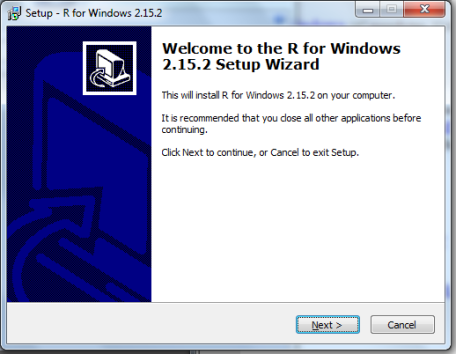
\includegraphics[scale=0.9]{images/1/install3-1.png}
	\end{center}
	Al dar siguiente estamos aceptando los términos de uso de la licencia GNU
	\begin{center}
		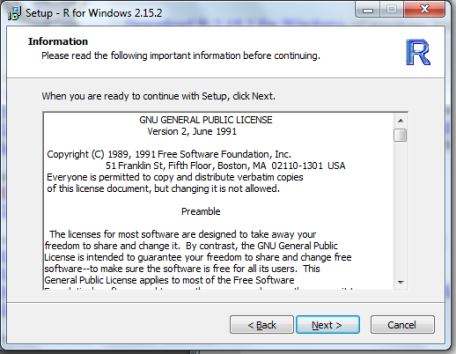
\includegraphics[scale=0.9]{images/1/install3-2.png}
	\end{center}
	, dependiendo de la arquitectura de su computador deberá elegir entre un tipo de instalación, usualmente el valor por defecto del instalador tiene la elección que requiere
	\begin{center}
		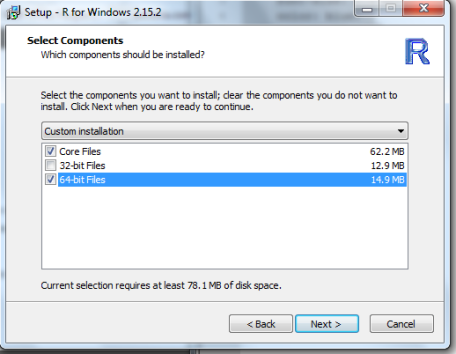
\includegraphics[scale=0.9]{images/1/install3-3.png}
	\end{center}
	En los siquientes pasos daremos siguiente, eventualmente llegaremos a
	\begin{center}
		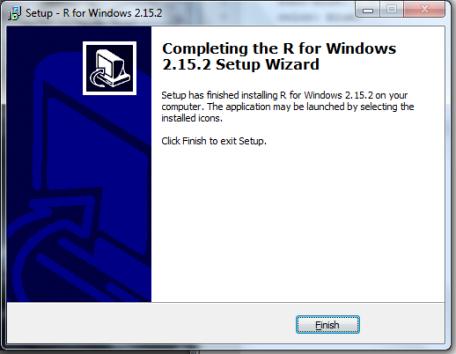
\includegraphics[scale=0.9]{images/1/install3-4.png}
	\end{center}
	Al finalizar, ya tendremos instalado R.
	\subsubsection{Instalación de R-studio}
	La instalación es muy sencilla, primero ejecute el .exe descargado en la página de R.
	\begin{center}
		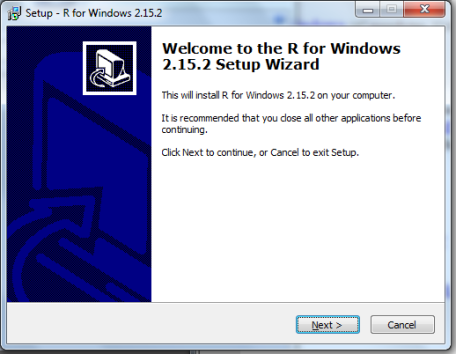
\includegraphics[scale=0.9]{images/1/install3-1.png}
	\end{center}
	Al dar siguiente estamos aceptando los términos de uso de la licencia GNU
	\begin{center}
		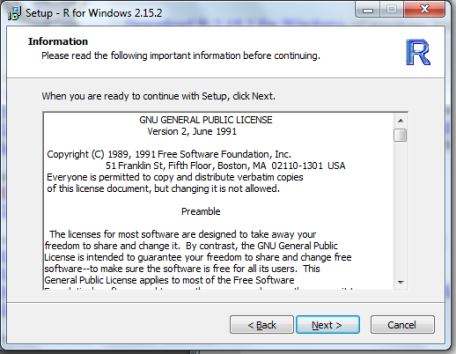
\includegraphics[scale=0.9]{images/1/install3-2.png}
	\end{center}
	, dependiendo de la arquitectura de su computador deberá elegir entre un tipo de instalación, usualmente el valor por defecto del instalador tiene la elección que requiere
	\begin{center}
		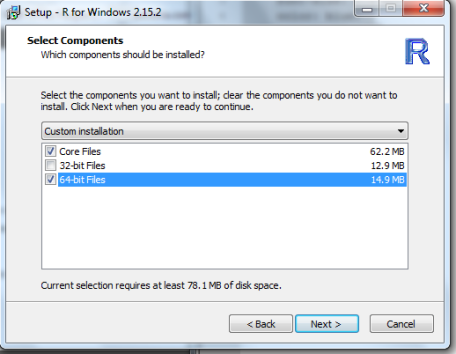
\includegraphics[scale=0.9]{images/1/install3-3.png}
	\end{center}
	En los siquientes pasos daremos siguiente, eventualmente llegaremos a
	\begin{center}
		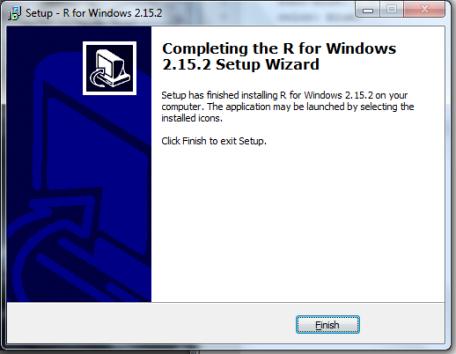
\includegraphics[scale=0.9]{images/1/install3-4.png}
	\end{center}
	Al finalizar, ya tendremos instalado R.
	\subsection{Descarga de Python}
	La instalación es muy sencilla, primero ejecute el .exe descargado en la página de R.
	\begin{center}
		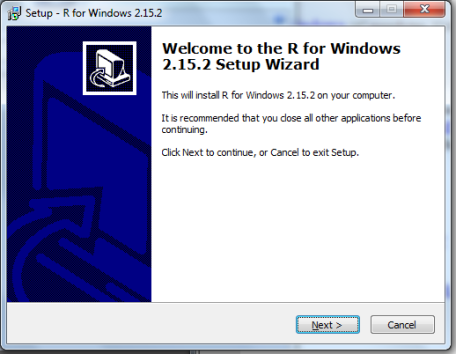
\includegraphics[scale=0.9]{images/1/install3-1.png}
	\end{center}
	Al dar siguiente estamos aceptando los términos de uso de la licencia GNU
	\begin{center}
		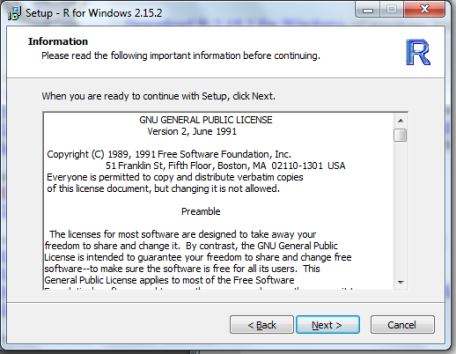
\includegraphics[scale=0.9]{images/1/install3-2.png}
	\end{center}
	, dependiendo de la arquitectura de su computador deberá elegir entre un tipo de instalación, usualmente el valor por defecto del instalador tiene la elección que requiere
	\begin{center}
		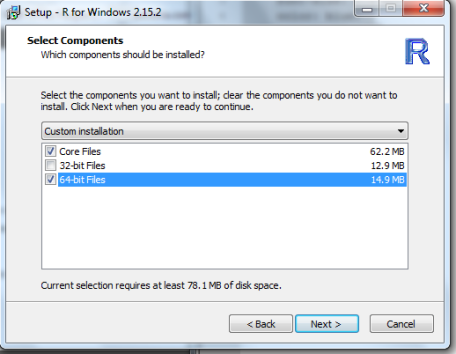
\includegraphics[scale=0.9]{images/1/install3-3.png}
	\end{center}
	En los siquientes pasos daremos siguiente, eventualmente llegaremos a
	\begin{center}
		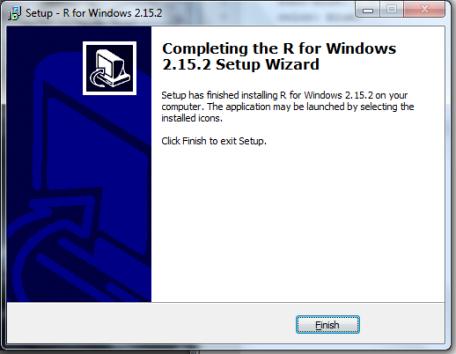
\includegraphics[scale=0.9]{images/1/install3-4.png}
	\end{center}
	Al finalizar, ya tendremos instalado R.
	\subsection{Código Fuente de los ejemplos presentados en el manual}
	Los fuentes de la construcción de este libro así como los ejemplos se encuentran en LINK DE GITHUB.
	\subsection{El lenguaje R}
	El lenguaje R es un lenguaje y entorno para el desarrollo de aplicaciones estadísticas, computacionales y gráficas.
	\paragraph{}R ofrece un amplio conjunto de herramientas estadísticas (para modelamiento, pruebas de hipótesis), herramientas gráficas y es altamente extensible, actualmente es uno de los proyectos de software libre más grandes del mundo, lo cual es una de sus fortalezas ya que al ser un proyecto de código abierto (en el que cualquiera puede aportar) toda la comunidad que utilza el software se beneficia de las contribuciones de todos, haciendo que R sea una herramienta en crecimiento y de uso extendido.
	\paragraph{} Este lenguaje tiene soporte para diferentes sistemas operativos.
	\subsubsection{El entorno}
	Cuando decimos que R también es un entorno, es debido a que no sólamente tiene las funciones que normalmente encontramos en un lenguaje de programación sino que también tiene un amplio abanico en crecimiento de 'paquetes'\footnote{Que son componentes adicionales que se pueden instalar según sea necesario.} para manipulación de texto, carga de archivos que a su vez pueden ser extendidas. R ha sido escrito deuna manera muy similar a los lenguajes de programación interpretados con el rendimiento del lenguaje de programación C.
	\subsubsection{Sintáxis}
	Como todo lenguaje debemos comprender algunas reglas básicas, a éstas reglas las conocemos como la sintáxis del lenguaje, dentro de esto encontramos varias categorías:
	\begin{itemize}
		\item \textbf{Definición y declaración de variables}. En todo lenguaje declaramos variables por lo que aprenderemos a definir variables junto con los tipos de datos en un programa R.
		\item \textbf{Operadores}. Repasaremos las operaciones básicas en R.
		\item \textbf{Estructuras de control}. Aquí ubicamos a las estructuras condicionales, condiciones en donde evaluamos el valor de verdad de una sentencia que permite alterar el flujo de un programa.
		\item  \textbf{Estructuras de repetición}. Aquí se encuentran las estructuras que nos permiten iterar, por ejemplo recorrer un archivo.
		\item \textbf{Funciones}. Son piezas de código, que nos ayudan a organizar el código. En general son una muy buena práctica de programación.
	\end{itemize}
	\subsubsection{Definición y declaración de variables}
	Primero repasaremos sobre los tipos de datos en R. R utiliza el paradigma de la orientación a objetos al límite, cada elemento en R es un objeto. R tiene $6$ tipos de datos:
	\begin{itemize}
		\item caracter. "a", "b", "hola"
		\item numérico. 2, 3, 3.14
		\item entero. 28L, 3L. el caracter L le indica a R que almacene el dato como un entero.
		\item lógico. TRUE, FALSE.
		\item complejo. 3+14i. En este manual no utilizaremos este tipo de datos para los problemas que manejamos es suficiente con los reales.
	\end{itemize}
	Ejemplo:
	\begin{verbatim}
		x <- "Hola"
		x
	\end{verbatim}
	Salida:
	\begin{verbatim}
		[1] "Hola"
	\end{verbatim}
	De esta forma acabamos de declarar una variable en R. Nótese que no fue necesario llevar a cabo una declaración del tipo de variable, R se encarga de asignar el tipo de dato dependiendo de lo que recibe. Por ejemplo:
	\begin{verbatim}
		x <- 1
		x
	\end{verbatim}
	Salida:
	\begin{verbatim}
		[1] 1
	\end{verbatim}
	
	Adicionalmente R también se encuentra provisto de funciones que nos permiten identificar propiedades de los objetos que declaramos:
	\begin{itemize}
		\item \texttt{class()}. Nos permite obtener la clase a la que está asociada a un objeto.
		\item \texttt{typeof()}. Nos permite obtener el tipo de dato de de una variable.
		\item \texttt{length()}. Nos permite obtener la longitud de un tipo de dato.
		\item \texttt{attributes()}. nos permite conocer si un objeto tiene determinados metadatos.
	\end{itemize}
	Ejemplo:
	\begin{verbatim}
		x <- 1L
		class(x)
		typeof(x)
		length(x)
		attributes(x)
	\end{verbatim}
	Salida:
	\begin{verbatim}
		class(x)
		[1] "integer"
		typeof(x)
		[1] "integer"
		length(x)
		[1] 1
		attributes(x)
		[1] NULL
	\end{verbatim}
	Cuando declaramos el tipo de dato sabíamos que era un entero, es por ello que obtenemos como tipo de dato y clase \texttt{integer}, como solo hemos ocupado 1 byte para almacenar el valor '1' obtenemos como valor de la función 1. Finalmente, \texttt{x} es un valor escalar, es por ello que no posee atributos y obtenemos el valor \texttt{NULL}, que indica que no tiene ningún atributo.
	\paragraph{} R cuenta con estructuras de datos para contener colecciones, nombraremos algunas de ellas:
	\begin{itemize}
		\item vectores atómicos.
		\item listas.
		\item matrices.
		\item data frame.
		\item factores.
	\end{itemize}
	En aplicaciones estadísticas encontraremos que es muy frecuente el uso de este tipo de estructuras.
	Los vectores se pueden declarar con varias funciones, las más comunes son \texttt{vector, logical, character, integer, numeric}.
	\paragraph{}Ejemplo:
	\begin{verbatim}
		vector()
		vector("character", length = 5)
	\end{verbatim}
	Salida
	\begin{verbatim}
		vector()
		[1] logical(0)
		vector("character", length = 5)
		[1] "" "" "" "" ""
	\end{verbatim}
	Con las funciones anteriores podemos analizar estos objetos.
	\paragraph{Matrices} las matrices son una extensión de los vectores pero tienen varias mas de una dimensión. Ejemplo:
	\begin{verbatim}
		m <- matrix(nrow = 2, ncol = 2)
		m
	\end{verbatim}
	Salida:
	\begin{verbatim}
			[,1]	[,2]
		[1,]	NA	NA
		[2,]	NA	NA
	\end{verbatim}
	\paragraph{Listas} Las listas en R actúan como contenedores. A diferencia de los vectores atómicos las listas puden contener diferentes tipos de datos, por ejemplo:
	\begin{verbatim}
		x <- list(1, "hola", TRUE, 3+14i)
		x	
	\end{verbatim}
	salida:
	\begin{verbatim}
		[[1]]
		[1] 1
		[[2]]
		[1] "hola"
		[[3]]
		[1] TRUE
		[[4]]
		[1] 3 + 14i
	\end{verbatim}
%%%%%%%%%%%%%%%%%%%%%%%%%%%%%%%%%%%%%%%%%%%%%%%%%%%%%%%%%%
	\section{Estadística Descriptiva}
	\subsection{Descripción}
	La \textit{estadística descriptiva} es la estadística que recolecta, presenta y caracteriza un conjunto de datos (por ejemplo, la edad de una población, la altura de los estudiantes de una escuela, temperatura en los meses de verano, etc.) con el fin de describir apropiadamente las diversas características de ese conjunto. Al conjunto de los distintos valores numéricos que adopta un carácter cuantitativo se llama variable estadística. Y existen de diferentes tipos. 
	\subsubsection{Tipos de variables}
	Las variables se clasifican de diversas maneras según el atributo que poseen, en estadística descriptiva se clasifican en:
	\begin{itemize}
		\item Variables cualitativas o categóricas, estas son las que no se pueden medir numéricamente (o de manera cuantitativa).
		\paragraph{Ejemplos}
		\begin{itemize}
			\item Nacionalidad.
			\item Color de piel.
			\item Sexo.
		\end{itemize}
		\item Variables cuantitativas, estas tienen un valor numérico. Son valores que podemos cuantificar y relacionar con un número.
		\paragraph{Ejemplos}
	\end{itemize}
	También se clasifican por su dimensión:
	\begin{itemize}
		\item Variables unidimensionales. Estas contienen la información sobre una característica.
		\paragraph{Ejemplos}
		\begin{itemize}
			\item Edad de los alumnos de una clase.
		\end{itemize}
		\item Variables bidimensionales. Estas contienen información sobre dos características de la población.
		\paragraph{Ejemplos}
		\begin{itemize}
			\item Edad y altura de los alumnos de una clase.
		\end{itemize}
		\item Variables pluridimensionales: recogen información sobre tres o más características.
		\paragraph{Ejemplo}
		\begin{itemize}
			\item Edad, altura y peso de los alumnos de una clase
		\end{itemize}
	\end{itemize}
	Para las varaiables cuantitativas existe una segunda categorización, esta se da según el tipo de número que contienen, estas pueden ser discretas o continuas.
	\begin{itemize}
		\item Las variables discretas son aquellas que sólo pueden tomar valores enteros $(1, 2, 8, -4, etc.)$
		\paragraph{Ejemplo}
		\begin{itemize}
			\item Número de hermanos, solo pueden ser $1, 2, 3 ... etc$ nunca podrá ser $3,45$.
		\end{itemize}
		\item Las variables continuas son aquellas que  pueden tomar cualquier valor real dentro de un intervalo.
		\paragraph{Ejemplo}
		\begin{itemize}
			\item La velocidad de un vehículo puede ser $90.4 km/h$, $94.57 km/h...etc$.
		\end{itemize}
	\end{itemize}
	\paragraph{} Cada variable tiene un comportamiento diferente y un tratamiento diferente, por lo que debemos aprender a reconocer algunas definiciones
	\paragraph{Individuo} Cualquier elemento que porte información sobre el fenómeno que se estudia. Así, si estudiamos la altura de los niños de una clase, cada alumno es un individuo; si se estudia el precio	de la vivienda, cada vivienda es un individuo.
	\paragraph{Población:} Es el conjunto de todos los individuos (personas, objetos, animales, etc.) que porten información sobre el fenómeno que se estudia. Por ejemplo, si se estudia el precio de la vivienda en una ciudad, la población será el total de las viviendas de dicha ciudad.
	\paragraph{Muestra} Es un subconjunto que seleccionado de una población. Por ejemplo, si se estudia el precio de la vivienda de una ciudad, lo normal será no recoger información sobre todas las viviendas de la ciudad (sería una labor muy compleja), sino que se suele seleccionar un subgrupo (muestra) que se entienda que es suficientemente representativo.
	\subsubsection{Datos y clasificación} Los datos pueden concebirse como información necesaria para ayudar a tomar una decisión con mayores fundamentos en una situación particular. Los datos son medidas y/o números recopilados a partir de la observación o instrumentos (como encuestas).  Existen varios métodos con los cuales se pueden obtener datos necesarios, se pueden buscar datos ya publicados por otras fuentes o publicaciones científicas.
	\begin{figure}[h!]
		\centering
		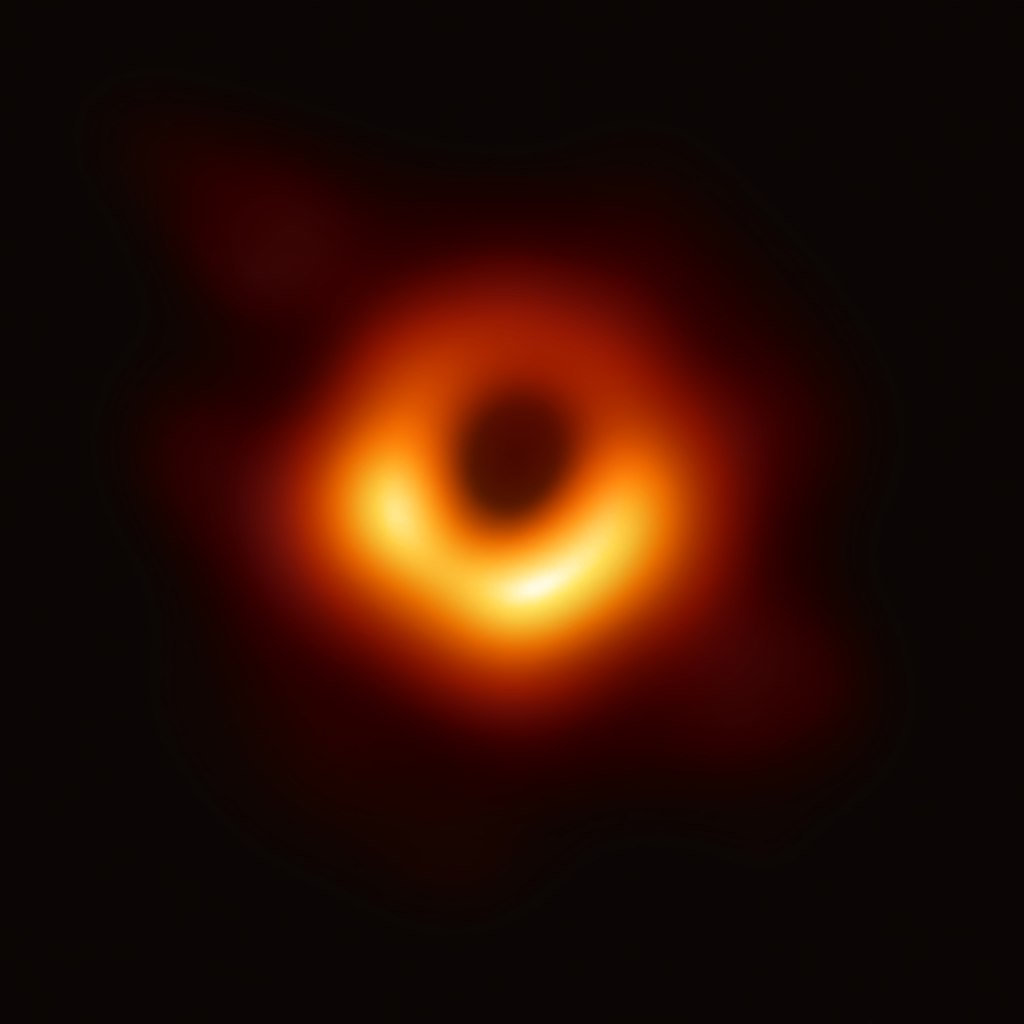
\includegraphics[width=0.5\linewidth]{images/2/black_hole.jpg}
		\caption[Agujero Negro M87]{En el centro de la galaxia M87, se encuentra este agujero negro supermasivo.}
	\end{figure}
	\subparagraph{Acerca de esta imágen} \textit{Para lograr la construcción de esta imágen se requirieron procesar mas de 5 Petabytes entre diversos observatorios. Ningún canal de comunicación sería eficiente para transportar esta cantidad de información, debido a ello se decidió enviar los discos duros en donde estaba almacenada la información recopilada, es un ejemplo muy claro de utilizar técnicas de recopilación de datos junto con modelos para construir y predecir una imágen de como se ve el agujero negro.}
	\paragraph{}También, se pueden diseñar experimentos y conducir estudios para recopilar los datos. En algunos casos se pueden hacer observaciones del comportamiento, actitudes y opiniones de los individuos en los que se está interesado en estudiar, en este caso se utilizan modelos matemáticos para construir un conjunto de datos.
	\paragraph{} Medir en el campo de las ciencias exactas es comparar una magnitud con otra, tomada de manera arbitraria como referencia, denominada patrón y expresar cuántas veces la contiene. En el campo de las ciencias sociales medir es “el proceso de vincular conceptos abstractos con indicadores empíricos”. Al resultado de medir se le llama medida.
	\paragraph{}La medición de las variables puede realizarse por medio de cuatro escalas de medición: la nominal, ordinal, de intervalo y de razón. Se utilizan para ayudar en la clasificación de las variables, el diseño de las preguntas para medir variables, e incluso indican el tipo de análisis estadístico apropiado para el tratamiento de los datos.\\
	\vspace{2mm}
	Una característica esencial de la medición es la dependencia que tiene de la posibilidad de variación. La validez y la confiabilidad de la medición de una variable depende de las decisiones que se tomen para operarla y lograr una adecuada comprensión del concepto evitando imprecisiones y ambigüedades, en caso  contrario, la variable corre el riesgo inherente de ser invalidada debido a que no produce información confiable.
	\begin{itemize}
		\item \textbf{Medición Nominal:}\\
		\vspace{2mm}
		En este nivel de medición se establecen categoría distintivas que no implican un orden específico. Por ejemplo, si la unidad de análisis es un grupo de personas, para clasificarlas se puede establecer la categoría sexo con dos niveles, masculino (M) y femenino (F), los encuestados sólo tienen que señalar su género, no se requiere de un orden real.\\
		\vspace{2mm}
		Así, se pueden asignar números a estas categorías para su identificación: $1=M$, $2=F$ o bien, se pueden invertir los números sin que afecte la medición: $1=F$ y $2=M$. En resumen en la escala nominal se asignan números a eventos con el propósito de identificarlos.
		\item  \textbf{Medición Ordinal:}\\ 
		\vspace{2mm}
		Se establecen categorías con dos o más niveles que implican un orden inherente entre si. La escala de medición ordinal es cuantitativa porque permite ordenar a los eventos en función de la mayor o menor  posesión de un atributo o característica. Por ejemplo, en las instituciones escolares de nivel básico suelen formar por estatura a los estudiantes, se desarrolla un orden cuantitativo pero no suministra medidas de los sujetos. Estas escalas admiten la asignación de números en función de un orden prescrito. Las formas más comunes de variables ordinales son ítems (reactivos) actitudinales estableciendo una serie de niveles que expresan una actitud de acuerdo o desacuerdo con respecto a algún referente. Por ejemplo, ante el reactivo: Pemex debe privatizarse, el respondiente puede marcar su
		respuesta de acuerdo a las siguientes alternativas:
		\begin{itemize}
			\item Totalmente de acuerdo.
			\item De acuerdo.
			\item Indiferente.
			\item En desacuerdo.
			\item Totalmente desacuerdo.
		\end{itemize}
		Las anteriores alternativas de respuesta pueden codificarse con números que van del uno al cinco que sugieren un orden preestablecido pero no implican una distancia entre un número y otro.
		\item  \textbf{Medición de Intervalo:}\\ 
		\vspace{2mm} 
		La medición de intervalo posee las características de la medición nominal y ordinal. Establece la distancia entre una medida y otra. La escala de intervalo se aplica a variables continuas pero carece de un punto cero absoluto. El ejemplo más representativo de este tipo de medición es un termómetro, cuando registra cero grados centígrados de temperatura indica el nivel de congelación del agua y cuando registra 100 grados centígrados indica el nivel de ebullición, el punto cero es arbitrario no real, lo que significa que en este punto no hay ausencia de temperatura. 
		\item \textbf{Medición de Razón:}\\
		\vspace{2mm}
		Una escala de medición de razón incluye las características de los tres anteriores niveles de medición (nominal, ordinal e intervalo). Determina la distancia exacta entre los intervalos de una categoría. Adicionalmente tiene un punto cero absoluto, es decir, en el punto cero no existe la característica o atributo que se mide. Las variables de ingreso, edad, número de hijos, etc. son ejemplos de este tipo de escala. El nivel de medición de razón se aplica tanto a variables continuas como discretas. 
	\end{itemize}
	
	\newpage
	\subsection{Medidas de tendencia central}
	Para cada ejemplo trabajaremos con los siguentes datos , importados de un excel a r. Lo haremos de la siguiente forma:
	\begin{lstlisting}[frame=single]
	library(readxl)
	## Libreria que lee los archivos 
	DB <- read_excel("C:/Nicolas/universidad/2019-2/Probabilidad
	y estadistica/baseDeDatos.xlsx", sheet = "BD CUALI - CUANTI")        
	## Ubicacion del archivo y que hoja quisiera importar 
	View(DB)
	\end{lstlisting}
	
	
	\subsubsection{Media o promedio}
	\vspace{2mm}
	La medida de tendencia central más conocida y utilizada es la media aritmética o promedio aritmético. Se representa por la letra griega $\mu$ cuando se trata del promedio del universo o población y por (léase Y barra) cuando se trata del promedio de la muestra. Es importante destacar que $\mu$ es una cantidad fija mientras que el promedio de la muestra es variable puesto que diferentes muestras extraídas de la misma población tienden a tener diferentes medias. La media se expresa en la misma unidad que los datos originales: centímetros, horas, gramos, etc.
	\vspace{2mm}
	\textbf{Ejemplo:}
	\vspace{1mm}
	Encontraremos la \textit{media} de una de las filas de los datos, obtaremos por hijos  en este caso debemos usar la transpuesta de la matrix para que el codigo funcióne lo cual se hará con el siguiente codigo:
	\begin{lstlisting}[frame=single]
	df<- baseDeDatos[,"Hijos"]
	dc<-t(df) ## Nos da la transpuesta del vector
	
	mean(dc)
	\end{lstlisting}
	En consola aparecera lo siguiente:
	
	\begin{center}
		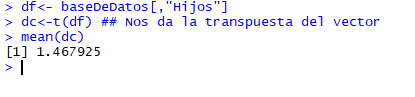
\includegraphics[]{media.PNG}
	\end{center}
	También se puede sacar la \textit{media recortada}, la cual recorta una proporción de observaciones por ambos lados de la distribución.
	\begin{lstlisting}[frame=single]
	df<- baseDeDatos[,"Hijos"]
	dc<-t(df) ## Nos da la transpuesta del vector
	
	mean(dc,trim = 0.2)
	\end{lstlisting}
	En consola aparecera lo siguiente:
	\begin{center}
		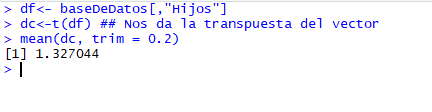
\includegraphics[]{mediaR.PNG}
	\end{center}
	\subsubsection{Mediana}
	Otra medida de tendencia central es la mediana. La mediana es el valor de la variable que ocupa la posición central, cuando los datos se disponen en orden de magnitud. Es decir, el 50\% de las observaciones tiene valores iguales o inferiores a la mediana y el otro 50\% tiene valores iguales o superiores a la mediana.\\
	\textbf{Ejemplo}\\
	\vspace{2mm}
	Encontraremos la \textit{mediana} de una de las filas de los datos, obtaremos por hijos  en este caso debemos usar la transpuesta de la matrix para que el codigo funcióne lo cual se hará con el siguiente codigo:
	\begin{lstlisting}[frame=single]
	df<- baseDeDatos[,"Hijos"]
	dc<-t(df) ## Nos da la transpuesta del vector
	
	median(dc)
	\end{lstlisting}
	En consola aparecera lo siguiente:
	\begin{center}
		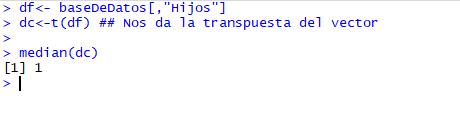
\includegraphics[]{Mediana.PNG}
	\end{center}
	\subsubsection{Moda}
	La moda de una distribución se define como el valor de la variable que más se repite. En un polígono de frecuencia la moda corresponde al valor de la variable que está bajo el punto más alto del gráfico. Una muestra puede tener más de una moda.\\
	\textbf{Ejemplo}\\
	\vspace{2mm}
	Encontraremos la \textit{moda} de una de las filas de los datos, obtaremos por hijos  en este caso debemos usar la transpuesta de la matrix para que el codigo funcióne lo cual se hará con el siguiente codigo:
	\begin{lstlisting}[frame=single]
	df<- baseDeDatos[,"Hijos"]
	dc<-t(df) ## Nos da la transpuesta del vector
	
	table(dc)
	\end{lstlisting}
	En consola aparecera lo siguiente:
	\begin{center}
		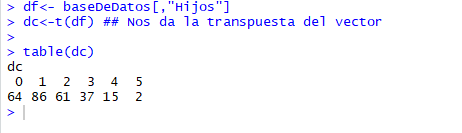
\includegraphics[]{Moda.PNG}
	\end{center}
	\subsection{Medidas de posición}
	\subsubsection{Cuartiles}
	Los cuartiles son los tres valores que dividen al conjunto de datos ordenados en cuatro partes porcentualmente iguales.
	Hay tres cuartiles denotados usualmente Q1, Q2, Q3. El segundo cuartil es precisamente la mediana. El primer cuartil, es el valor en el cual o por debajo del cual queda un cuarto (25\%) de todos los valores de la sucesión (ordenada); el tercer cuartil, es el valor en el cual o por debajo del cual quedan las tres cuartas partes (75\%) de los datos.\textbf{Ejemplo}\\
	\vspace{2mm}
	Encontraremos los \textit{cuartiles} de una de las filas de los datos, obtaremos por hijos  en este caso debemos usar la transpuesta de la matrix para que el codigo funcióne lo cual se hará con el siguiente codigo:
	\begin{lstlisting}[frame=single]
	df<- baseDeDatos[,"Hijos"]
	dc<-t(df) ## Nos da la transpuesta del vector
	
	quantile(dc)
	\end{lstlisting}
	En consola aparecera lo siguiente:
	\begin{center}
		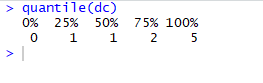
\includegraphics[]{Cuartiles.PNG}
	\end{center}
	\subsubsection{Percentiles}
	Los percentiles son, tal vez, las medidas más utilizadas para propósitos de ubicación o clasificación de las personas cuando atienden características tales como peso, estatura, etc. 
	Los percentiles son ciertos números que dividen la sucesión de datos ordenados en cien partes porcentualmente iguales. Estos son los 99 valores que dividen en cien partes iguales el conjunto de datos ordenados. Los percentiles (P1, P2,... P99), leídos primer percentil,..., percentil 99.\\
	\textbf{Ejemplo}\\
	\vspace{2mm}
	Encontraremos los \textit{percentiles} de una de las filas de los datos, obtaremos por hijos  en este caso debemos usar la transpuesta de la matrix para que el codigo funcióne lo cual se hará con el siguiente codigo:
	\begin{lstlisting}[frame=single]
	df<- baseDeDatos[,"Hijos"]
	dc<-t(df) ## Nos da la transpuesta del vector
	
	quantile(dc, 0.25)
	\end{lstlisting}
	En consola aparecera lo siguiente:
	\begin{center}
		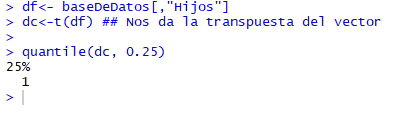
\includegraphics[]{Percentiles.PNG}
	\end{center}
	
	\subsection{Medidas de dispersión}
	\subsubsection{Rango}
	El Rango es el intervalo entre el valor máximo y el valor mínimo; por ello, comparte unidades con los datos. Permite obtener una idea de la dispersión de los datos, cuanto mayor es el rango, más dispersos están los datos (sin considerar la afectación de los valores extremos). El rango, también es llamado amplitud o recorrido.\\
	\textbf{Ejemplo}\\
	\vspace{2mm}
	Encontraremos el \textit{rango} de una de las filas de los datos, obtaremos por hijos  en este caso debemos usar la transpuesta de la matrix para que el codigo funcióne lo cual se hará con el siguiente codigo:
	\begin{lstlisting}[frame=single]
	df<- baseDeDatos[,"Hijos"]
	dc<-t(df) ## Nos da la transpuesta del vector
	
	range(dc)
	\end{lstlisting}
	En consola aparecera lo siguiente:
	\begin{center}
		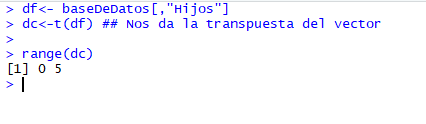
\includegraphics[]{Rango.PNG}
	\end{center}
	
	\subsubsection{Desviación estandar}
	La desviación estándar es la medida de dispersión más común, que indica qué tan dispersos están los datos con respecto a la media. Mientras mayor sea la desviación estándar, mayor será la dispersión de los datos.\newpage
	\textbf{Ejemplo}\\
	\vspace{2mm}
	Encontraremos la \textit{desviasión estandar} de una de las filas de los datos, obtaremos por hijos  en este caso debemos usar la transpuesta de la matrix para que el codigo funcióne lo cual se hará con el siguiente codigo:
	\begin{lstlisting}[frame=single]
	df<- baseDeDatos[,"Hijos"]
	dc<-t(df) ## Nos da la transpuesta del vector
	
	sd(dc)
	
	\end{lstlisting}
	En consola aparecera lo siguiente:
	\begin{center}
		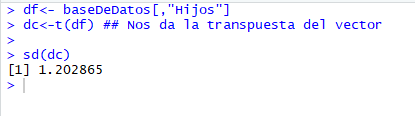
\includegraphics[]{Desviacion_estandar.PNG}
	\end{center}
	
	\subsubsection{Varianza}
	La varianza mide qué tan dispersos están los datos alrededor de la media. La varianza es igual a la desviación estándar elevada al cuadrado.\\
	\textbf{Ejemplo}\\
	\vspace{2mm}
	Encontraremos la \textit{varianza} de una de las filas de los datos, obtaremos por hijos lo cual se hará con el siguiente codigo:
	\begin{lstlisting}[frame=single]
	df<- baseDeDatos[,"Hijos"]
	
	var(df)
	\end{lstlisting}
	En consola aparecera lo siguiente:
	\begin{center}
		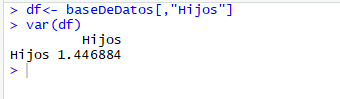
\includegraphics[]{Varianza.PNG}
	\end{center}
	
	\subsubsection{Coeficiente de variación}
	El coeficiente de variación permite comparar las dispersiones de dos distribuciones distintas, siempre que sus medias sean positivas.\newpage
	\textbf{Ejemplo}\\
	\vspace{2mm}
	Encontraremos el \textit{coeficiente de variación} de una de las filas de los datos, obtaremos por hijos  en este caso debemos usar la transpuesta de la matrix para que el codigo funcióne lo cual se hará con el siguiente codigo:
	\begin{lstlisting}[frame=single]
	df<- baseDeDatos[,"Hijos"]
	dc<-t(df) ## Nos da la transpuesta del vector
	
	CV <- function(dc){sd(dc)*100/mean(dc)}
	CV(dc)
	
	
	
	\end{lstlisting}
	En consola aparecera lo siguiente:
	\begin{center}
		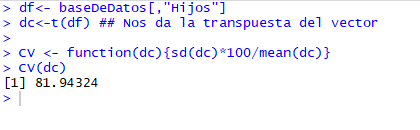
\includegraphics[]{Coeficiente_varianza.PNG}
	\end{center}
	
	Se calcula para cada una de las distribuciones y los valores que se obtienen se comparan entre sí.
	
	La mayor dispersión corresponderá al valor del coeficiente de variación mayor.
	%%%%   Hasta deje el día sabado %%%%%
	
	%%%%%% Adiciones al manual %%%%%%%%%
	\subsubsection{Error estándar}
	\subsection{Tablas}
	\subsubsection{Frecuencia absoluta}
	La frecuencia absoluta es una medida estadística que nos da información acerca de la cantidad de veces que se repite un suceso al realizar un número determinado de experimentos aleatorios.\\
	\textbf{Ejemplo}\\
	\vspace{2mm}
	Encontraremos la \textit{tabla de frecuencia absoluta} de una de las filas de los datos, obtaremos por hijos  en este caso debemos usar la transpuesta de la matrix para que el codigo funcióne lo cual se hará con el siguiente codigo:
	\begin{lstlisting}[frame=single]
	df<- baseDeDatos[,"Hijos"]
	dc<-t(df) ## Nos da la transpuesta del vector
	
	table(dc)
	\end{lstlisting}
	En consola aparecera lo siguiente:
	\begin{center}
		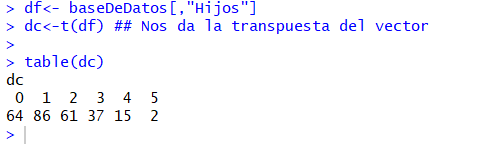
\includegraphics[width = \linewidth]{TFabsoluta.PNG}
	\end{center}
	\subsubsection{Frecuencia relativa}
	La frecuencia relativa es el cociente entre la frecuencia absoluta de un determinado valor y el número total de datos.\\
	\textbf{Ejemplo}\\
	\vspace{2mm}
	Encontraremos la \textit{tabla de frecuencia relativa} de una de las filas de los datos, obtaremos por hijos  en este caso debemos usar la transpuesta de la matrix para que el codigo funcióne lo cual se hará con el siguiente codigo:
	\begin{lstlisting}[frame=single]
	df<- baseDeDatos[,"Hijos"]
	dc<-t(df) ## Nos da la transpuesta del vector
	
	table(dc)/length(dc)
	\end{lstlisting}
	En consola aparecera lo siguiente:
	\begin{center}
		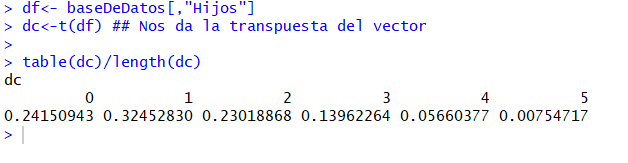
\includegraphics[width=\linewidth]{TFrelativa.PNG}
	\end{center}
	\subsubsection{Frecuencia absoluta acumulada}
	La frecuencia absoluta acumulada es el resultado de ir sumando las frecuencias absolutas de las observaciones o valores de una población o muestra.\\
	\textbf{Ejemplo}\\
	\vspace{2mm}
	Encontraremos la \textit{tabla de frecuencia absoluta acumulada} de una de las filas de los datos, obtaremos por hijos  en este caso debemos usar la transpuesta de la matrix para que el codigo funcióne lo cual se hará con el siguiente codigo:
	\begin{lstlisting}[frame=single]
	df<- DB[,"Hijos"]
	dc<-t(df) ## Nos da la transpuesta del vector
	
	cumsum(table(dc))
	\end{lstlisting}
	En consola aparecera lo siguiente:
	\begin{center}
		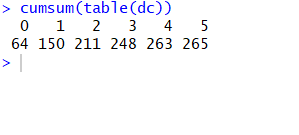
\includegraphics[]{TFabsolutaAcum.PNG}
	\end{center}
	
	\subsubsection{Frecuencia relativa acumulada}
	La frecuencia relativa acumulada es el resultado de ir sumando las frecuencias absolutas de las observaciones o valores de una población o muestra.\\
	\textbf{Ejemplo}\\
	\vspace{2mm}
	Encontraremos la \textit{tabla de frecuencia relativa acumulada} de una de las filas de los datos, obtaremos por hijos  en este caso debemos usar la transpuesta de la matrix para que el codigo funcióne lo cual se hará con el siguiente codigo:
	\begin{lstlisting}[frame=single]
	df<- DB[,"Hijos"]
	dc<-t(df) ## Nos da la transpuesta del vector
	
	cumsum(table(dc)/length(dc))
	\end{lstlisting}
	En consola aparecera lo siguiente:
	\begin{center}
		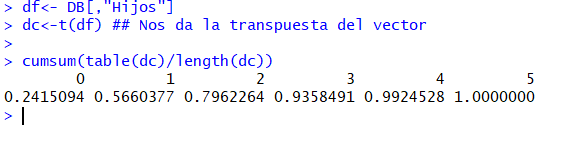
\includegraphics[width=\linewidth]{TFrelativaAcum.PNG}
	\end{center}
	\newpage
	\subsection{Graficas}
	Para las gráficas usaremos el paquete \textit{ggplot2}, se mostrara el uso de cada una de las gráficas, si no tenemos el paquete intalado podemos usar el siguente comando:
	
	\begin{lstlisting}[frame=single]
	if(!any(grepl("ggplot2",installed.packages()))){
	install.packages("ggplot2",dependencies = TRUE)
	}
	\end{lstlisting}
	\subsubsection{Barras}
	Un diagrama de barras, también conocido como gráfico de barras o gráfico de columnas, es una forma de representar gráficamente un conjunto de datos o valores, y está conformado por barras rectangulares de longitudes proporcionales a los valores representados. Los gráficos de barras son usados para comparar cantidades de valores en diferentes momentos, o también podría decirse productos. Las barras pueden orientarse horizontal o verticalmente.\\
	\textbf{Ejemplo}\\
	Realizaremos un diagrama de \textit{barras} a la variable hijos, genero y estado civil el cual ser relizara con el siguiente código:
	\begin{lstlisting}[frame=single]
	library(ggplot2)
	
	df<- baseDeDatos
	
	ggplot(data=df, aes(x=Genero
	, y=Hijos, fill = Estado_Civil)) + 
	geom_bar(stat="identity", position="dodge")
	\end{lstlisting}
	En plots aparecera lo siguiente:
	\begin{center}
		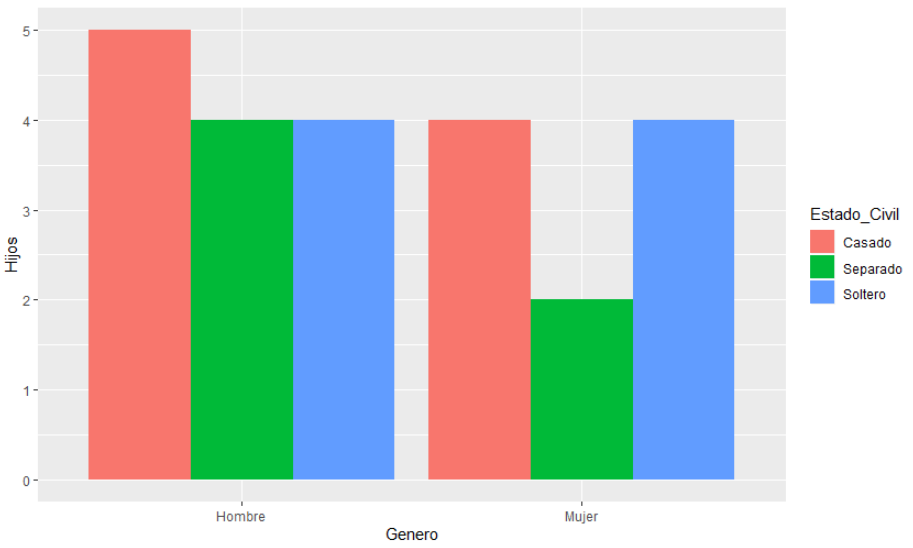
\includegraphics[width = 14cm]{GraficaBarras.PNG}
	\end{center}
	
	
	\subsubsection{Barras apliladas}
	Gráfica que apila una serie de rectángulos (uno sobre otro), en donde el área de cada rectángulo es proporcional a la cantidad que representa. Este tipo de gráfica puede utilizarse para comparar fácilmente las partes de un todo.\\
	\textbf{Ejemplo}\\
	Realizaremos un diagrama de \textit{barras apiladas} a las variables hijos, genero y estado civil el cual ser relizara con el siguiente código:
	\begin{lstlisting}[frame=single]
	library(ggplot2)
	
	df<-baseDeDatos
	
	ggplot(data=df, aes(x=Genero
	, y=Hijos, fill = Estado_Civil)) + 
	geom_bar(stat="identity", position="stack")
	\end{lstlisting}
	En plots aparecera lo siguiente:
	\begin{center}
		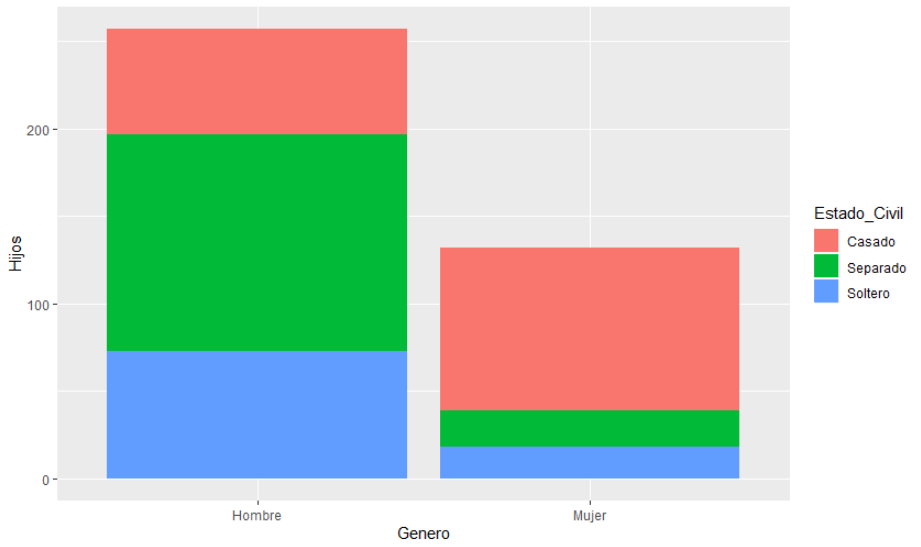
\includegraphics[width = 14cm]{GraficaBarrasA.PNG}
	\end{center}
	
	\subsubsection{Pie}
	Un gráfico circular o gráfica circular, también llamado "gráfico de pastel", "gráfico de tarta", "gráfico de torta" o "gráfica de 360 grados", es un recurso estadístico que se utiliza para representar porcentajes y proporciones. El número de elementos comparados dentro de una gráfica circular suele ser de más de cuatro.\newpage
	\textbf{Ejemplo}\\
	Realizaremos un diagrama de \textit{pie} a la variable Accidentes el cual ser relizara con el siguiente código:
	\begin{lstlisting}[frame=single]
	library(ggplot2)
	df<- baseDeDatos
	
	accidentes <- df$ACCIDENTE
	pie <- function(x) {
	title <- deparse(substitute(x))
	
	x <- data.frame(modality = na.omit(x))
	library(dplyr)
	
	Df <- x %>% group_by(modality) %>% summarise(frequency=n()) %>%
	arrange(desc(frequency))
	
	Df$modality <- ordered(Df$modality, levels 
	= unlist(Df$modality, use.names = F))
	
	Df <- Df %>%
	arrange(desc(modality)) %>%
	mutate( prop = frequency/sum(frequency)*100 
	, lab.ypos = cumsum(prop) - 0.5*prop)
	
	mycols <- c("#0073C2FF", "#EFC000FF", "#868686FF", "#CD534CFF")
	
	g <- ggplot(Df, aes(x = "", y = prop, fill = modality)) +
	geom_bar(width = 1, stat = "identity", color = "white") +
	coord_polar("y", start = 0)+
	geom_text(aes(y = lab.ypos
	, label = paste(prop,"%")), color = "white")+
	scale_fill_manual(values = mycols) +
	theme_void()
	
	return(g)
	}
	pie(accidentes)
	\end{lstlisting}
	En plots aparecera lo siguiente:
	\begin{center}
		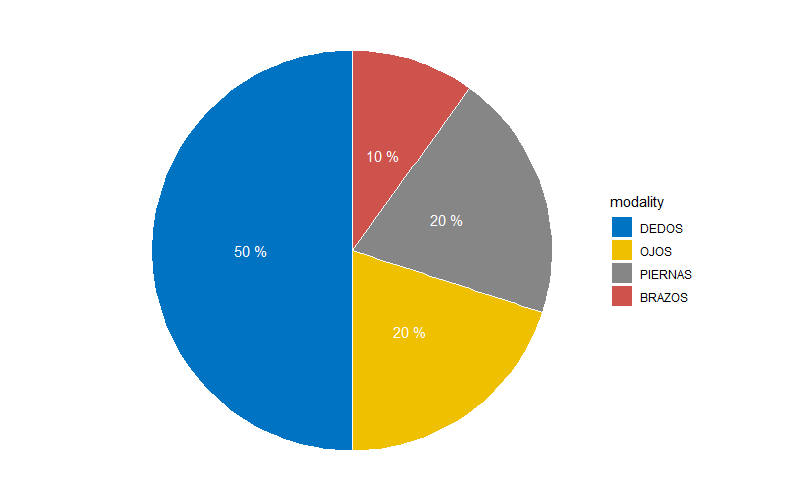
\includegraphics[width = 14cm]{GC.png}
	\end{center}
	
	\subsubsection{Boxplot}
	Los diagramas de Caja-Bigotes (boxplots o box and whiskers) son una presentación visual que describe varias características importantes, al mismo tiempo, tales como la dispersión y simetría.
	
	Para su realización se representan los tres cuartiles y los valores mínimo y máximo de los datos, sobre un rectángulo, alineado horizontal o verticalmente.\\
	\textbf{Ejemplo}\\
	Realizaremos un  \textit{boxplot} a las variables hijos y genero el cual ser relizara con el siguiente código:
	\begin{lstlisting}[frame=single]
	library(ggplot2)
	
	df<- baseDeDatos
	
	ggplot(data=df, aes(x=Genero, y=Hijos)) + 
	geom_boxplot() +
	guides(fill=FALSE)
	\end{lstlisting}
	En plots aparecera lo siguiente:
	\begin{center}
		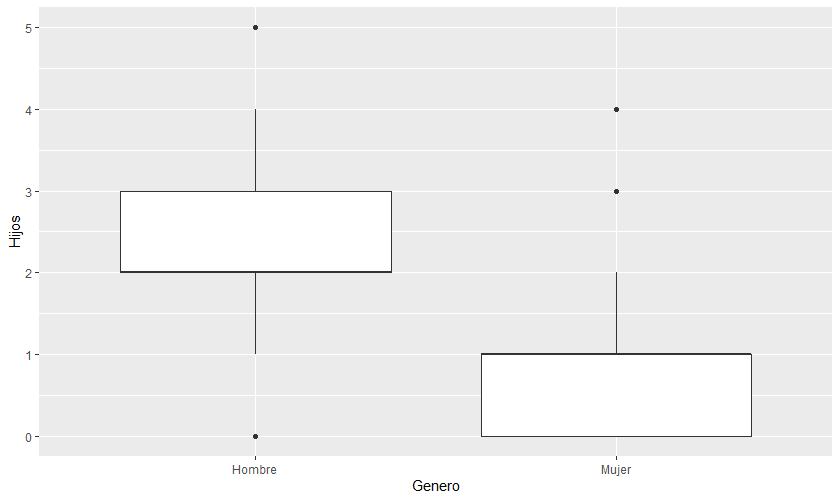
\includegraphics[width = 14cm]{GaficaBox.png}
	\end{center}
	
	\subsubsection{Histograma}
	Un histograma es una representación gráfica de una variable en forma de barras, donde la superficie de cada barra es proporcional a la frecuencia de los valores representados. Sirven para obtener una "primera vista" general, o panorama, de la distribución de la población, o de la muestra, respecto a una característica, cuantitativa y continua (como la longitud o el peso).\\
	\textbf{Ejemplo}\\
	Realizaremos un \textit{histograma} a la variable hijos, el cual ser relizara con el siguiente código:
	\begin{lstlisting}[frame=single]
	df<- DB[,"Hijos"]
	dc <- t(df)
	
	
	hist(x = dc,
	probability= TRUE,
	xlab = "Hijos", ylab = "Fracuencia",
	col = c("blue","red","yellow"),
	main = "Histograma Hijos")
	lines(density(dc), lwd = 2)
	lines(density(dc),
	col = "black", lty = 2, ps = 20)
	\end{lstlisting}
	En plots aparecera lo siguiente:
	\begin{center}
		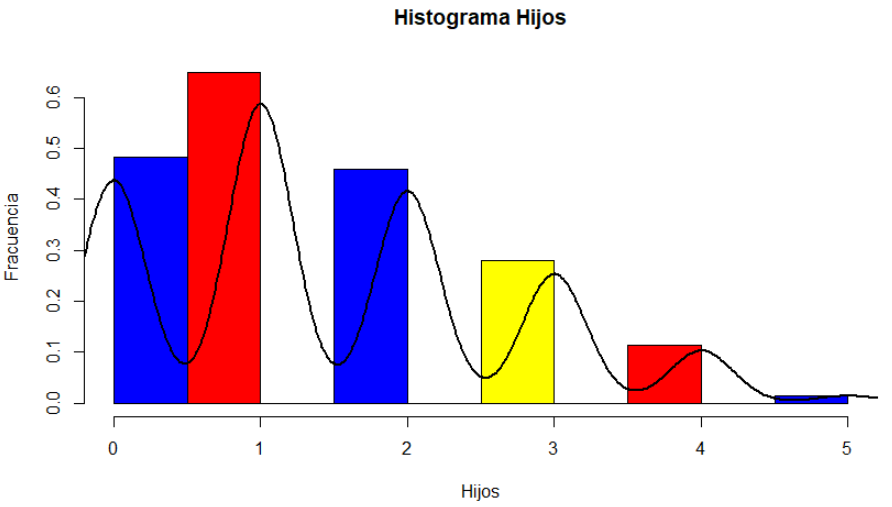
\includegraphics[width = 14cm]{GraficaHisto.PNG}
	\end{center}
	\subsubsection{Pareto}
	El diagrama de Pareto, también llamado curva cerrada o Distribución A-B-C, es una gráfica para organizar datos de forma que estos queden en orden descendente, de izquierda a derecha y separados por barras. Permite asignar un orden de prioridades. El diagrama permite mostrar gráficamente el principio de Pareto (pocos vitales, muchos triviales), es decir, que hay muchos problemas sin importancia frente a unos pocos muy importantes. Mediante la gráfica colocamos los "pocos que son vitales" a la izquierda y los "muchos triviales" a la derecha.\\
	\textbf{Ejemplo}\\
	Realizaremos un \textit{pareto} a la variable accidentes, el cual ser relizara con el siguiente código:
	\begin{lstlisting}[frame=single]
	install.packages("qcc")
	library(ggplot2)
	library(qcc)
	
	df <- baseDeDatos
	dc<- (df)
	table <- table(dc)
	pareto.chart(table)
	\end{lstlisting}
	En consola nos mostrara lo siguente:
	\begin{center}
		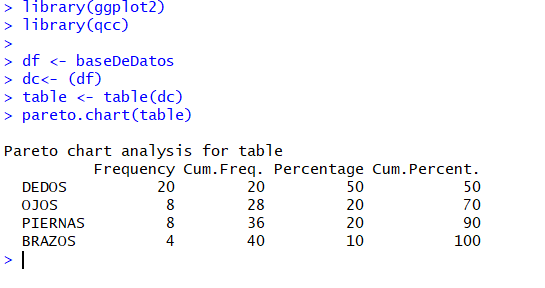
\includegraphics[]{imgPareto.PNG}
	\end{center}
	En plots aparecera lo siguiente:
	\begin{center}
		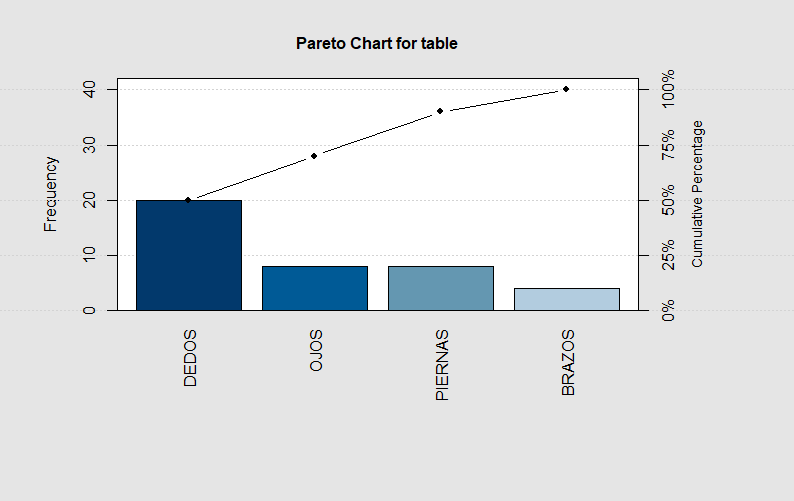
\includegraphics[width = 15cm]{Gpareto.png}
	\end{center}
%%%%%%%%%%%%%%%%%%%%%%%%%%%%%%%%%%%%%%%%%%%%%%%%%%%%%%%%%%
\end{document}